\let\negmedspace\undefined
\let\negthickspace\undefined
\documentclass[journal]{IEEEtran}
\usepackage[a5paper, margin=10mm, onecolumn]{geometry}
%\usepackage{lmodern} % Ensure lmodern is loaded for pdflatex
\usepackage{tfrupee} % Include tfrupee package

\setlength{\headheight}{1cm} % Set the height of the header box
\setlength{\headsep}{0mm}     % Set the distance between the header box and the top of the text

\usepackage{gvv-book}
\usepackage{gvv}
\usepackage{cite}
\usepackage{amsmath,amssymb,amsfonts,amsthm}
\usepackage{algorithmic}
\usepackage{graphicx}
\usepackage{textcomp}
\usepackage{xcolor}
\usepackage{txfonts}
\usepackage{listings}
\usepackage{enumitem}
\usepackage{mathtools}
\usepackage{gensymb}
\usepackage{comment}
\usepackage[breaklinks=true]{hyperref}
\usepackage{tkz-euclide} 
\usepackage{listings}
% \usepackage{gvv}                                        
\def\inputGnumericTable{}                                 
\usepackage[latin1]{inputenc}                                
\usepackage{color}                                            
\usepackage{array}                                            
\usepackage{longtable}                                       
\usepackage{calc}                                             
\usepackage{multirow}                                         
\usepackage{hhline}                                           
\usepackage{ifthen}                                           
\usepackage{lscape}
\begin{document}

\bibliographystyle{IEEEtran}
\vspace{3cm}

\title{9.7.4}
\author{EE24BTECH11012 - Bhavanisankar G S}
% \maketitle
% \newpage
% \bigskip
{\let\newpage\relax\maketitle}

\renewcommand{\thefigure}{\theenumi}
\renewcommand{\thetable}{\theenumi}
\setlength{\intextsep}{10pt} % Space between text and floats


\numberwithin{equation}{enumi}
\numberwithin{figure}{enumi}
\renewcommand{\thetable}{\theenumi}

\textbf{QUESTION} : \\
Prove that $x^2 - y^2 = c\brak{x^2 + y^2}^2$ is the general solution of differential equation, $\brak{x^3 - 3xy^2} dx = \brak{y^3 - 3x^2y} dy$, where $c$ is a parameter. Considering $y(1) = 1$, find the particular solution of the given differential equation.\\
\textbf{SOLUTION} : \\
\begin{align}
	\brak{x^3 - 3xy^2} dx &= \brak{y^3 - 3x^2y} dy \\
	\frac{dy}{dx} &= \frac{x^3 - 3xy^2}{y^3 - 3x^2y} \label{eq:de} 
\end{align}
Putting 
\begin{align}
	y &= vx \label{eq:sub}
\end{align}
in \eqref{eq:de}, we have
\begin{align}
	v + x \frac{dv}{dx} &= \frac{1 - 3v^2}{v^3 - 3v} \\
	x \frac{dv}{dx} &= \frac{1 - v^4}{v^3 - 3v}
\end{align}
\textbf{Separating the variables}, we have
\begin{align}
	\frac{v^3 - 3v}{1 - v^4} dv &= \frac{1}{x} dx 
\end{align}
By the method of \textbf{partial fractions}, we have
\begin{align}
	\brak{\frac{-2v}{1 + v^2} - \frac{v}{1 - v^2}} dv &= \frac{1}{x} dx \label{eq:sim}
\end{align}
Integrating on both the sides of \eqref{eq:sim}, we have
\begin{align}
	\int \brak{\frac{-2v}{1 + v^2} - \frac{v}{1 - v^2}} dv &= \int \frac{1}{x} dx \\
	\log \brak{\frac{\sqrt{1 - v^2}}{1 + v^2}} &= \log{x} + \log{c},  c - \text{ constant } \\
	\brak{\frac{\sqrt{1 - v^2}}{1 + v^2}} &= cx \label{eq:ans}
\end{align}
Substituting \eqref{eq:sub} in \eqref{eq:ans} and rearranging, we have
\begin{align}
	\frac{\sqrt{x^2 - y^2}}{x^2 + y^2} &= c \\
	x^2 - y^2 &= c \brak{x^2 + y^2}^2
\end{align}
Hence proved. \\
Substituting the initial conditions ,we have \\
\begin{align}
	1 - 1 &= c(1 + 1) \\
	c &= 0
\end{align}
\textbf{Particular solution} : \\
\begin{align}
	x^2 - y^2 &= 0 \\
	y &= \pm x 
\end{align}
By the \textbf{Forward-Euler method}, we have \\
\begin{align}
	f^{\prime} (x) &= \lim_{h \to 0} \frac{f(x+h) - f(x)}{h} \\
	f^{\prime} (x) &\approx \frac{f(x+h) - f(x)}{h} \text{ for small } h\\
	y_{n+1} &\approx y_{n} + h \brak{y^{\prime}} \label{eq:dif}
\end{align}
Substituting \eqref{eq:de} in \eqref{eq:dif}, we have 
\begin{align}
	y_{n+1} &= y_{n} + h \brak{\frac{x_{n}^3 - 3x_{n}y_{n}^2}{y_{n}^3 - 3x_{n}^2y_{n}}} \label{eq:lab}
\end{align}
which is the required difference equation. \\
\textbf{Algorithm} : \\
Take
\begin{align}
	x_0 &= 1 \\
	y_0 &= 1 \\
	h &= 0.01 
\end{align}
The simulation plot can be plotted by iterating $y_{n}$ ( \eqref{eq:lab} ) for different $x_{n}$ as
\begin{align}
	x_{n+1} &= x_{n} + h 
\end{align}
The plot for computational and theoritical solution are given below.
\begin{figure}[h]
				 \centering
				 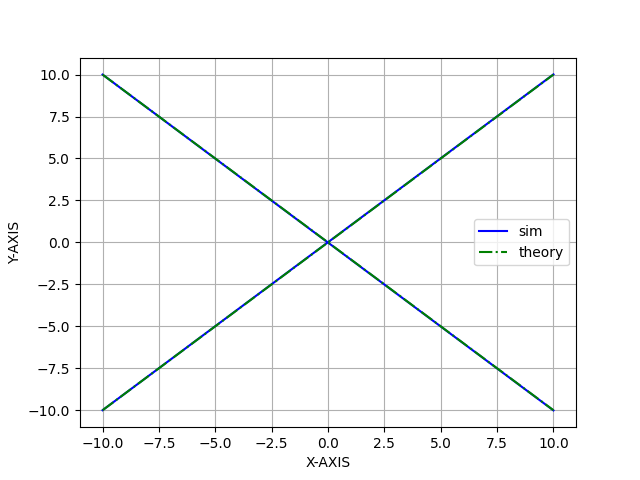
\includegraphics[width=\columnwidth]{figs/fig1.png}
				 \caption{Computational and theoritical solution.}
				 \label{fig:Plot1} 
			 \end{figure}



	
\end{document}
